% ========================================
% Chapter 3 Figures - SwarmGuard Methodology
% Beautiful TikZ Diagrams for Thesis
% ========================================

\documentclass[12pt,a4paper]{article}

% Required Packages
\usepackage[utf8]{inputenc}
\usepackage[margin=0.5in]{geometry}
\usepackage{tikz}
\usetikzlibrary{shapes.geometric, arrows.meta, positioning, backgrounds, shadows, patterns, decorations.pathmorphing, fit, calc}
\usepackage{xcolor}

% Color Scheme - Professional and Modern
\definecolor{primaryblue}{RGB}{41, 128, 185}
\definecolor{secondarygreen}{RGB}{39, 174, 96}
\definecolor{accentorange}{RGB}{230, 126, 34}
\definecolor{alertred}{RGB}{192, 57, 43}
\definecolor{lightgray}{RGB}{236, 240, 241}
\definecolor{darkgray}{RGB}{52, 73, 94}
\definecolor{purple}{RGB}{142, 68, 173}
\definecolor{teal}{RGB}{22, 160, 133}

% TikZ Styles
\tikzset{
    node box/.style={
        rectangle,
        rounded corners=3mm,
        draw=darkgray,
        very thick,
        minimum width=3cm,
        minimum height=1.2cm,
        align=center,
        drop shadow={opacity=0.3},
        font=\sffamily\bfseries
    },
    worker node/.style={
        node box,
        fill=primaryblue!20,
        draw=primaryblue,
        text=darkgray
    },
    master node/.style={
        node box,
        fill=alertred!20,
        draw=alertred,
        text=darkgray
    },
    component/.style={
        rectangle,
        rounded corners=2mm,
        draw=teal,
        thick,
        minimum width=2.5cm,
        minimum height=0.8cm,
        align=center,
        fill=teal!10,
        font=\sffamily\small
    },
    database/.style={
        cylinder,
        cylinder uses custom fill,
        cylinder body fill=purple!20,
        cylinder end fill=purple!40,
        draw=purple,
        thick,
        minimum width=2cm,
        minimum height=1.5cm,
        align=center,
        font=\sffamily\small,
        drop shadow={opacity=0.2}
    },
    arrow/.style={
        -Stealth,
        thick,
        draw=darkgray
    },
    metric arrow/.style={
        -Stealth,
        thick,
        draw=secondarygreen,
        dashed
    },
    alert arrow/.style={
        -Stealth,
        very thick,
        draw=alertred
    },
    api arrow/.style={
        -Stealth,
        thick,
        draw=primaryblue,
        dotted
    },
    state/.style={
        circle,
        draw=primaryblue,
        very thick,
        minimum size=2.5cm,
        align=center,
        fill=primaryblue!10,
        font=\sffamily\bfseries\small,
        drop shadow={opacity=0.3}
    },
    transition/.style={
        -Stealth,
        thick,
        draw=darkgray,
        font=\sffamily\tiny,
        align=center
    }
}

\begin{document}

\pagestyle{empty}

% ========================================
% FIGURE 3.1: System Architecture
% ========================================

\begin{figure}[p]
\centering
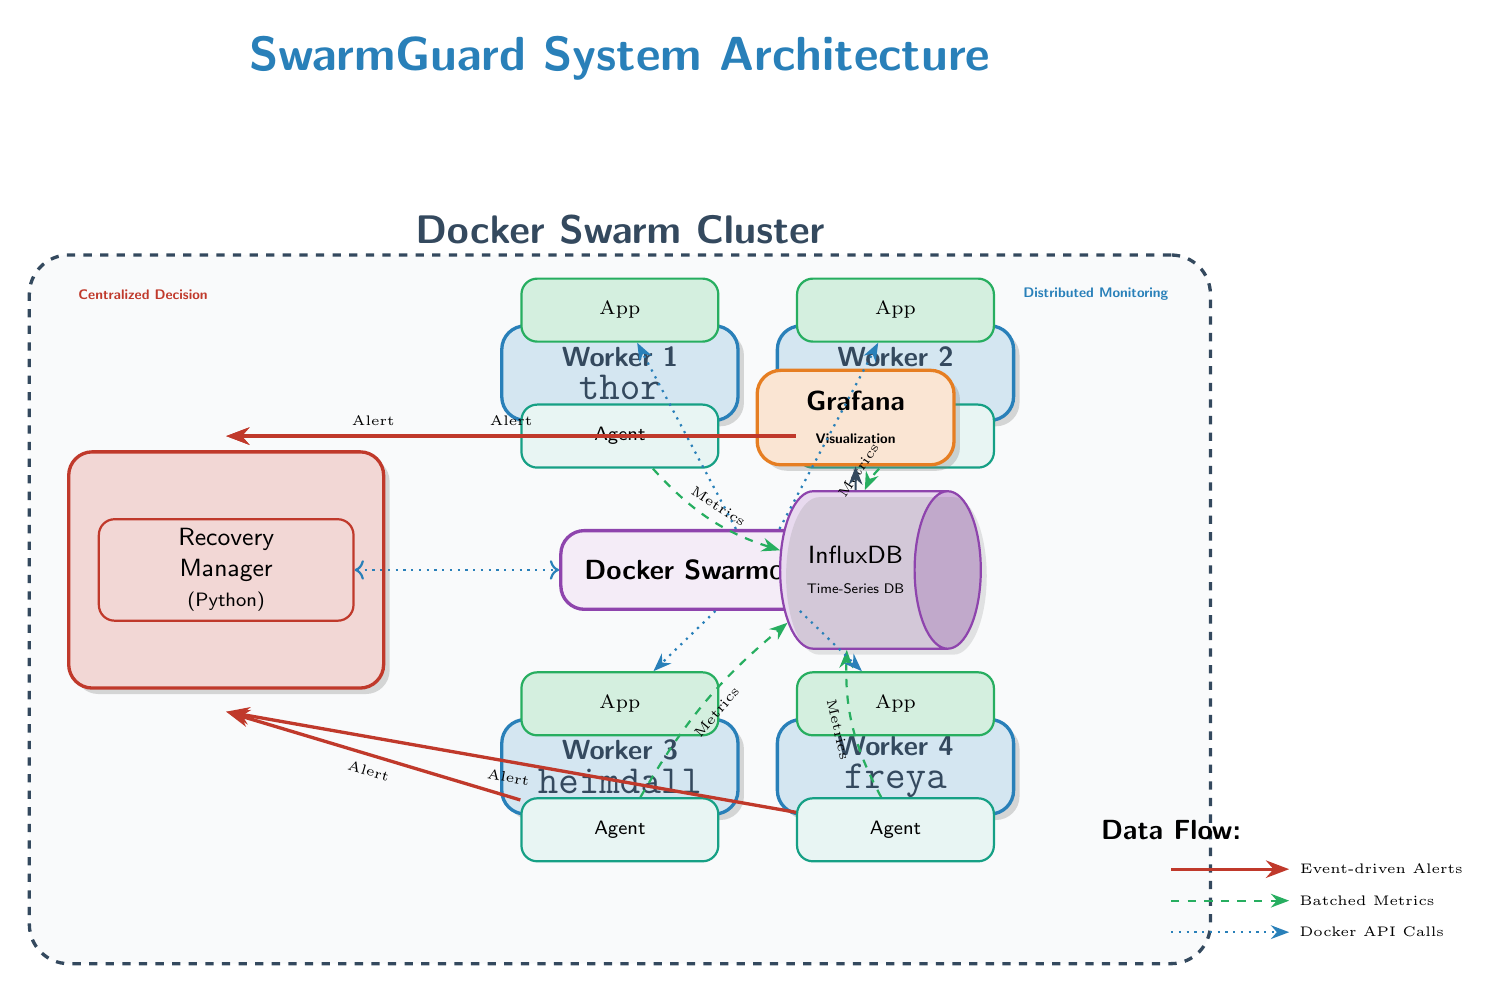
\begin{tikzpicture}[node distance=1.5cm and 2cm]

% Title
\node[font=\LARGE\bfseries\sffamily, text=primaryblue] at (0, 8) {SwarmGuard System Architecture};

% Docker Swarm Cluster Background
\begin{scope}[on background layer]
    \node[draw=darkgray, very thick, rounded corners=5mm, dashed,
          fill=lightgray!30, minimum width=15cm, minimum height=9cm,
          label={[font=\Large\bfseries\sffamily, text=darkgray]above:Docker Swarm Cluster}]
          at (0, 1) {};
\end{scope}

% Master Node (Odin)
\node[master node, minimum width=4cm, minimum height=3cm] (master) at (-5, 1.5) {
    Master Node\\
    \Large\texttt{odin}
};

% Recovery Manager inside Master
\node[component, fill=alertred!20, draw=alertred, text width=3cm]
     (recovery) at (-5, 1.5) {
    Recovery\\Manager\\
    \scriptsize (Python)
};

% Worker Nodes
\node[worker node] (worker1) at (0, 4) {Worker 1\\\Large\texttt{thor}};
\node[worker node] (worker2) at (3.5, 4) {Worker 2\\\Large\texttt{loki}};
\node[worker node] (worker3) at (0, -1) {Worker 3\\\Large\texttt{heimdall}};
\node[worker node] (worker4) at (3.5, -1) {Worker 4\\\Large\texttt{freya}};

% Monitoring Agents in Workers
\node[component] (agent1) at (0, 3.2) {\scriptsize Agent};
\node[component] (agent2) at (3.5, 3.2) {\scriptsize Agent};
\node[component] (agent3) at (0, -1.8) {\scriptsize Agent};
\node[component] (agent4) at (3.5, -1.8) {\scriptsize Agent};

% Application Containers
\node[component, fill=secondarygreen!20, draw=secondarygreen, font=\scriptsize]
     (app1) at (0, 4.8) {App};
\node[component, fill=secondarygreen!20, draw=secondarygreen, font=\scriptsize]
     (app2) at (3.5, 4.8) {App};
\node[component, fill=secondarygreen!20, draw=secondarygreen, font=\scriptsize]
     (app3) at (0, -0.2) {App};
\node[component, fill=secondarygreen!20, draw=secondarygreen, font=\scriptsize]
     (app4) at (3.5, -0.2) {App};

% Docker Swarm Orchestration Layer
\node[draw=purple, very thick, rounded corners=3mm, fill=purple!10,
      minimum width=5cm, minimum height=1cm, font=\sffamily\bfseries]
     (swarm) at (1.75, 1.5) {
    Docker Swarm\\
    \scriptsize Orchestration API
};

% InfluxDB + Grafana (Outside Cluster)
\node[database, right=5cm of master] (influx) {
    InfluxDB\\
    \tiny Time-Series DB
};

\node[node box, fill=accentorange!20, draw=accentorange,
      minimum width=2.5cm, minimum height=1.2cm, above=0.3cm of influx]
     (grafana) {
    Grafana\\
    \tiny Visualization
};

% === ARROWS AND DATA FLOW ===

% Alerts: Agents → Recovery Manager
\draw[alert arrow] (agent1) -- node[above, sloped, font=\tiny] {Alert} (-5, 3.2);
\draw[alert arrow] (agent2) -- node[above, sloped, font=\tiny] {Alert} (-5, 3.2);
\draw[alert arrow] (agent3) -- node[below, sloped, font=\tiny] {Alert} (-5, -0.3);
\draw[alert arrow] (agent4) -- node[below, sloped, font=\tiny] {Alert} (-5, -0.3);

% Metrics: Agents → InfluxDB (batched)
\draw[metric arrow, bend right=15] (agent1) to node[above, sloped, font=\tiny] {Metrics} (influx);
\draw[metric arrow, bend right=10] (agent2) to node[above, sloped, font=\tiny] {Metrics} (influx);
\draw[metric arrow, bend left=10] (agent3) to node[below, sloped, font=\tiny] {Metrics} (influx);
\draw[metric arrow, bend left=15] (agent4) to node[below, sloped, font=\tiny] {Metrics} (influx);

% Grafana reads from InfluxDB
\draw[arrow] (influx) -- (grafana);

% Recovery Manager ↔ Docker Swarm API
\draw[api arrow, <->] (recovery) -- (swarm);

% Docker Swarm manages containers
\draw[api arrow] (swarm) -- (app1);
\draw[api arrow] (swarm) -- (app2);
\draw[api arrow] (swarm) -- (app3);
\draw[api arrow] (swarm) -- (app4);

% Legend
\begin{scope}[shift={(7, -3)}]
    \node[font=\sffamily\bfseries] at (0, 1.2) {Data Flow:};
    \draw[alert arrow] (0, 0.7) -- ++(1.5, 0) node[right, font=\tiny] {Event-driven Alerts};
    \draw[metric arrow] (0, 0.3) -- ++(1.5, 0) node[right, font=\tiny] {Batched Metrics};
    \draw[api arrow] (0, -0.1) -- ++(1.5, 0) node[right, font=\tiny] {Docker API Calls};
\end{scope}

% Annotations
\node[font=\tiny\sffamily, text=alertred, anchor=west] at (-7, 5) {
    \textbf{Centralized Decision}
};
\node[font=\tiny\sffamily, text=primaryblue, anchor=west] at (5, 5) {
    \textbf{Distributed Monitoring}
};

\end{tikzpicture}
\caption{SwarmGuard System Architecture showing distributed monitoring agents, centralized recovery manager, Docker Swarm orchestration, and observability stack.}
\label{fig:architecture}
\end{figure}

\clearpage

% ========================================
% FIGURE 3.2: Zero-Downtime Migration Timeline
% ========================================

\begin{figure}[p]
\centering
\begin{tikzpicture}[
    scale=0.95,
    timeline/.style={-Stealth, very thick, draw=darkgray},
    event/.style={circle, fill=primaryblue, inner sep=2pt},
    milestone/.style={rectangle, rounded corners=2mm, draw=darkgray, thick,
                     fill=white, align=center, font=\sffamily\small, minimum height=0.8cm},
    task box/.style={rectangle, rounded corners=2mm, thick, align=center,
                    font=\sffamily\small, minimum width=3cm, minimum height=1.2cm,
                    drop shadow={opacity=0.2}}
]

% Title
\node[font=\LARGE\bfseries\sffamily, text=primaryblue] at (7, 8) {Zero-Downtime Migration Timeline};

% Timeline axis
\draw[timeline] (0, 0) -- (14, 0) node[right, font=\sffamily\bfseries] {Time};

% Time markers
\foreach \x/\label in {0/T+0ms, 2/T+100ms, 4/T+2000ms, 7/T+5000ms, 10/T+6000ms, 13/T+8000ms} {
    \draw[thick] (\x, -0.1) -- (\x, 0.1);
    \node[below, font=\tiny\sffamily] at (\x, -0.2) {\label};
}

% === EVENTS ===

% T+0: Alert Reception
\node[event] (e0) at (0, 0) {};
\node[milestone, fill=alertred!20, above=0.5cm of e0] (m0) {
    Alert\\Reception
};
\draw[arrow] (e0) -- (m0);

% T+100ms: Constraint Application
\node[event] (e1) at (2, 0) {};
\node[milestone, fill=accentorange!20, above=0.5cm of e1] (m1) {
    Constraint\\Applied
};
\draw[arrow] (e1) -- (m1);

% T+2000ms: New Task Start
\node[event] (e2) at (4, 0) {};
\node[milestone, fill=secondarygreen!20, above=0.5cm of e2] (m2) {
    New Task\\Starts
};
\draw[arrow] (e2) -- (m2);

% T+5000ms: New Task Healthy
\node[event] (e3) at (7, 0) {};
\node[milestone, fill=secondarygreen!30, above=0.5cm of e3] (m3) {
    New Task\\Healthy
};
\draw[arrow] (e3) -- (m3);

% T+6000ms: Old Task Termination
\node[event] (e4) at (10, 0) {};
\node[milestone, fill=darkgray!20, above=0.5cm of e4] (m4) {
    Old Task\\Terminates
};
\draw[arrow] (e4) -- (m4);

% T+8000ms: Migration Complete
\node[event] (e5) at (13, 0) {};
\node[milestone, fill=purple!20, above=0.5cm of e5] (m5) {
    Migration\\Complete
};
\draw[arrow] (e5) -- (m5);

% === TASK LIFECYCLES ===

% Old Task (Red)
\node[task box, fill=alertred!30, draw=alertred, text width=5.5cm]
     (old_task) at (2, -2.5) {
    \textbf{Old Task (worker-2)}\\
    \scriptsize Running → Draining → Shutdown
};
\draw[very thick, alertred] (0, -2.5) -- (10, -2.5);
\node[font=\tiny, text=alertred, left] at (0, -2.5) {Running};
\node[font=\tiny, text=alertred, right] at (10, -2.5) {Stopped};

% New Task (Green)
\node[task box, fill=secondarygreen!30, draw=secondarygreen, text width=5.5cm]
     (new_task) at (8.5, -4) {
    \textbf{New Task (worker-3)}\\
    \scriptsize Starting → Healthy → Running
};
\draw[very thick, secondarygreen] (4, -4) -- (13, -4);
\node[font=\tiny, text=secondarygreen, left] at (4, -4) {Created};
\node[font=\tiny, text=secondarygreen, right] at (13, -4) {Running};

% === ZERO-DOWNTIME WINDOW ===

% Highlight concurrent execution period
\fill[secondarygreen!10, opacity=0.5] (4, -5.5) rectangle (10, 2);
\draw[very thick, secondarygreen, dashed] (4, -5.5) -- (4, 2);
\draw[very thick, secondarygreen, dashed] (10, -5.5) -- (10, 2);

\node[font=\Large\bfseries\sffamily, text=secondarygreen, anchor=south]
     at (7, 2.2) {
    \textbf{ZERO-DOWNTIME WINDOW}
};

\node[font=\footnotesize\sffamily, text=secondarygreen, align=center]
     at (7, -5.8) {
    Both tasks running concurrently\\
    Service continuously available
};

% === SERVICE AVAILABILITY INDICATOR ===

\node[font=\sffamily\bfseries] at (14, -6.5) {Service:};
\draw[very thick, secondarygreen] (0, -7) -- (13, -7);
\node[font=\tiny, text=secondarygreen, left] at (0, -7) {✓ Available};
\node[font=\tiny, text=secondarygreen, right] at (13, -7) {✓ Available};

% Annotations
\draw[<->, thick, primaryblue] (4, 1.8) -- (10, 1.8)
    node[midway, above, font=\small\sffamily\bfseries] {4 seconds overlap};

\end{tikzpicture}
\caption{Zero-downtime migration timeline showing concurrent execution of old and new tasks between T+2000ms and T+6000ms, ensuring continuous service availability.}
\label{fig:migration_timeline}
\end{figure}

\clearpage

% ========================================
% FIGURE 3.3: Horizontal Scaling State Machine
% ========================================

\begin{figure}[p]
\centering
\begin{tikzpicture}[
    node distance=4cm and 3.5cm,
    scale=0.9,
    transform shape
]

% Title
\node[font=\LARGE\bfseries\sffamily, text=primaryblue] at (0, 7) {Horizontal Scaling State Machine};

% === STATES ===

% Normal State (1 replica)
\node[state, fill=secondarygreen!20, draw=secondarygreen] (normal) at (-5, 3) {
    Normal\\
    ────\\
    1 Replica\\
    \tiny Load < 70\%
};

% High Load Detection
\node[state, fill=accentorange!20, draw=accentorange] (high_load) at (0, 3) {
    High Load\\
    Detected\\
    ────\\
    \tiny Breach Count: 2
};

% Scaled State (2+ replicas)
\node[state, fill=primaryblue!20, draw=primaryblue, minimum size=3cm] (scaled) at (5, 3) {
    Scaled\\
    ────\\
    2+ Replicas\\
    \tiny Load Distributed
};

% Load Decrease Detection
\node[state, fill=accentorange!20, draw=accentorange] (low_load) at (5, -1.5) {
    Load\\
    Decreased\\
    ────\\
    \tiny Idle Detected
};

% Cooldown Period
\node[state, fill=purple!20, draw=purple] (cooldown) at (0, -1.5) {
    Cooldown\\
    Period\\
    ────\\
    \tiny 180s Wait
};

% === TRANSITIONS ===

% Normal → High Load Detection
\draw[transition, bend left=15] (normal) to node[above, sloped] {
    CPU > 75\% \textbf{AND}\\
    Network > 65 Mbps
} (high_load);

% High Load → Scale-Up Decision → Scaled
\draw[transition, very thick, secondarygreen] (high_load) to node[above, sloped] {
    \textbf{SCALE UP}\\
    \tiny replicas = n + 1
} (scaled);

% Scaled → Low Load (loop)
\draw[transition, bend left=20] (scaled) to node[right, sloped] {
    Load < 70\%\\
    \tiny (sustained)
} (low_load);

% Low Load → Cooldown
\draw[transition] (low_load) to node[below, sloped] {
    Mark Idle\\
    \tiny Start Timer
} (cooldown);

% Cooldown → Normal (Scale-Down)
\draw[transition, very thick, alertred, bend right=20] (cooldown) to node[below, sloped] {
    \textbf{SCALE DOWN}\\
    \tiny replicas = n - 1\\
    \tiny (after 180s)
} (normal);

% Cooldown → Scaled (Load Returns)
\draw[transition, bend right=15, dashed] (cooldown) to node[above, sloped, align=center] {
    Load Increases\\
    \tiny Cancel Scale-Down
} (scaled);

% Self-loops
\draw[transition, loop above, looseness=8] (normal) to node[above, align=center] {
    \tiny Normal Operation\\
    \tiny Monitor Metrics
} (normal);

\draw[transition, loop above, looseness=8] (scaled) to node[above, align=center] {
    \tiny Serving Traffic\\
    \tiny Monitor Usage
} (scaled);

% === ANNOTATIONS ===

% Scenario 2 Trigger
\node[draw=accentorange, very thick, rounded corners=3mm, fill=accentorange!10,
      align=center, font=\footnotesize\sffamily, minimum width=3.5cm,
      drop shadow={opacity=0.2}]
     at (-5, 0.5) {
    \textbf{Scenario 2 Trigger:}\\
    \tiny High CPU/Memory\\
    \tiny + High Network
};

% Oscillation Prevention
\node[draw=purple, very thick, rounded corners=3mm, fill=purple!10,
      align=center, font=\footnotesize\sffamily, minimum width=3.5cm,
      drop shadow={opacity=0.2}]
     at (0, -4.5) {
    \textbf{Oscillation Prevention:}\\
    \tiny Conservative 180s cooldown\\
    \tiny prevents thrashing
};

% Success Metrics
\node[draw=secondarygreen, very thick, rounded corners=3mm, fill=secondarygreen!10,
      align=center, font=\footnotesize\sffamily, minimum width=3.5cm,
      drop shadow={opacity=0.2}]
     at (5, 0) {
    \textbf{Success Metrics:}\\
    \tiny Scale-up: 6-8s median\\
    \tiny Load distribution: 50/50
};

% Legend
\begin{scope}[shift={(-5, -5)}]
    \node[font=\sffamily\bfseries] at (0, 0.5) {Legend:};
    \draw[transition, very thick, secondarygreen] (0, 0) -- ++(1.2, 0)
        node[right, font=\tiny] {Scale-Up Action};
    \draw[transition, very thick, alertred] (0, -0.4) -- ++(1.2, 0)
        node[right, font=\tiny] {Scale-Down Action};
    \draw[transition, dashed] (0, -0.8) -- ++(1.2, 0)
        node[right, font=\tiny] {Conditional Transition};
\end{scope}

\end{tikzpicture}
\caption{Horizontal scaling state machine showing transitions between normal operation, high load detection, scaled state, and cooldown period with 180-second oscillation prevention.}
\label{fig:scaling_state_machine}
\end{figure}

\end{document}
